%%%%%%%%%%%%%%%%%%%%%%%%%%%%%%%%%%%%%%%%%%%%%%%%%%%%%%%%%%%%%%%%%%%%%%%%%%%%%%%%%%%%%%%%%%%%%%%%%%%%

\chapter{The interstellar medium}
\chaptermark{the instellar medium}
\label{introduction: chapter: ism}

%%%%%%%%%%%%%%%%%%%%%%%%%%%%%%%%%%%%%%%%%%%%%%%%%%%%%%%%%%%%%%%%%%%%%%%%%%%%%%%%%%%%%%%%%%%%%%%%%%%%

Galaxies are complex objects build from dark matter and various phases of baryonic matter \citep[e.g.][]{1933AcHPh...6..110Z}. The different constituents are in constant interplay through gravitational, electro-magnetic and mechanical forces. 
The interstellar medium (ISM) is a cardinal point is these interactions \citep[e.g.][]{2016SAAS...43...85K} as the ISM contains large amounts of mass, stars form from it and return gas and energy to the ISM. 
A lack of suitable ISM can starve star formation and galaxy evolution but also boost it to extreme conditions.
In such violent environments, the ISM can even be expelled from its host galaxy and into the intergalactic medium \citep[e.g.][]{1971ApJ...165..381J}.

The term interstellar medium encompasses all baryonic matter between stars. This includes gas of various types and dust but also radiation is often considered a part of the ISM.
The ISM in early type (ellipticals) and irregular galaxies can be very different from the ISM in late type (spiral) galaxies. For now, we focus on the ISM in typical spiral, star-forming galaxies.


%%%%%%%%%%%%%%%%%%%%%%%%%%%%%%%%%%%%%%%%%%%%%%%%%%%%%%%%%%%%%%%%%%%%%%%%%%%%%%%%%%%%%%%%%%%%%%%%%%%%

\section{Phases of the ISM}
\label{introdution: section: ism: phases}

The ISM consists of several phases that are commonly grouped according to temperature and composition \citep[e.g.][]{2011piim.book.....D}.
\vspace{0.5\baselineskip}

\emph{Hot ionized medium} --- By volume, most ($\sim 50$\%) of the gas trapped by the gravity of a galaxy and its dark matter halo is hot ($T \GTRSIM 10^{5.5}$\,K). Heated by shocks and ionized by collisions, this phase is very thin ($n \LESS 0.01$ atoms per cubic cm).
\vspace{0.5\baselineskip}

\emph{Warm ionized medium} --- At lower temperatures of $T \sim 10^4$\,K, this phase typically fills $\sim10$\% of a galaxy's volume. Energetic photons from the galaxy provide the heating and ionize the gas. Its density is typically of order 1\,\pcm3.
\vspace{0.5\baselineskip}

\emph{Warm neutral medium} --- This phase is cool enough ($\sim 5000$\,K) to remain neutral. At $\sim 40$\% volume filling fraction, it overlaps spatially with warm and hot ionized medium. Its density of $\sim 1$\,\pcm3 and the large filling fraction shows that there can be substantial amounts of gas in this phase.
%The 21\,cm line of neutral hydrogen (\hi) is the main tracer of the warm neutral medium.
\vspace{0.5\baselineskip}

\emph{Cold neutral medium} --- Although virtually identical in composition to the warm neutral medium, the cold neutral medium is much colder ($T \sim 100$\,K) and denser (order of 30\,\pcm3). This is only possible due to shielding from radiation by outer gas layers in relatively compact aggregations. These clouds, therefore, occupy a small volume in a galaxy ($\sim 1$\%) primarily in a thin and thick disk, typically co-planar to the stellar disk.
\vspace{0.5\baselineskip}

\emph{Cold molecular medium} --- Only a tiny volume fraction of $\sim 0.1$\% of a spiral galaxy is filled by molecular gas. Shielding by layers of neutral gas are required to intercept radiation (electro-magnetic and cosmic rays) that can easily destroy molecular bonds. Within (giant) molecular clouds, the gas can efficiently cool down to $T \LESSSIM 100$\,K and may even reach $T \LESSSIM 10$\,K. The densities in molecular clouds range from hundreds to $\GTR 10^8$\,\pcm3 which can be enough to start gravitational collapse under its own weight in the star formation process (Chapter~\ref{introduction: chapter: star formation}).
\vspace{0.5\baselineskip}

The ISM phases are not stationary but in constant interaction and evolution. Heating and cooling can transfer mass, momentum and energy between the phases. Molecular gas can be dissociated and ionized by intense radiation and its constituent atoms feed the warm and hot ISM phases. Vice versa, ionized gas can recombine with electrons, radiatively cool and form molecules or even dust to replenish the cold ISM phases.

Typically, the ISM phases are roughly in pressure equilibrium. The thermal pressure is usually weak while magnetic and turbulent pressure dominate.
Gas not in equilibrium can be found as e.g. self-gravitating molecular gas (Section~\ref{introduction: section: star formation: sketch}) or outflows (Section~\ref{introduction: section: star formation: outflows}).


%%%%%%%%%%%%%%%%%%%%%%%%%%%%%%%%%%%%%%%%%%%%%%%%%%%%%%%%%%%%%%%%%%%%%%%%%%%%%%%%%%%%%%%%%%%%%%%%%%%%

\section{Elements in the ISM}
\label{introdution: section: ism: elements}

From Big Bang nucleosynthesis, hydrogen is the most common element in the universe with $\sim 90$\% abundance, followed by helium with $\sim 10$\% \citep[e.g.][]{1994ARA&A..32..191W}. Hence, the ISM phases are also dominated by hydrogen in the forms of ionized (\hii), neutral (\hi) and molecular (\htwo) hydrogen.
However, the heavy elements that were almost exclusively cooked up by stars \citep[e.g.][]{1988ccna.book.....R,2014PASA...31...30K}, are an important addition to the ISM. Their wide repertoire of electronic transitions allow for much more efficient cooling than pure hydrogen and helium, and thus regulate the heating/cooling of the ISM.
The most common elements in the ISM aside from hydrogen and helium are low atomic number elements, alpha elements with multiples of four atomic numbers (C, N, O, Ne, Mg, Si, S, Ar, Ca, Ti) and elements of the iron peak (Ti, V, Cr, Mn, Fe, Co, Ni) \citep[e.g.][]{1994ARA&A..32..191W}. 
Alpha elements are efficiently produced by alpha (helium core) capture in core-collapse (type II) supernovae while iron peak elements are synthesized alongside alpha elements in type Ia supernovae.
Hence, different forms of these elements provide crucial tracers to study the ISM. For instance, the spectral lines of ionized and neutral heavy elements reveal the hot and warm phases of the ISM. In the molecular phase, complex compounds with dozens of atoms can form and offer an overwhelming amount of spectral lines to study chemistry and physical conditions \citep[e.g.][]{1973ApJ...185..505H}. In dust grains, thousands to millions of atoms and molecules agglomerate and provide a surface for chemical reactions that cannot take place in the gas phase \citep[e.g.][]{2017MolAs...9....1W,2005JPhCS...6...18H}.


%%%%%%%%%%%%%%%%%%%%%%%%%%%%%%%%%%%%%%%%%%%%%%%%%%%%%%%%%%%%%%%%%%%%%%%%%%%%%%%%%%%%%%%%%%%%%%%%%%%%

\section{Molecular clouds}
\label{introdution: section: ism: molecular clouds}

Molecular gas typically resides in so-called molecular clouds of diffuse, filamentary and/or concentrated structures of various sizes. Most of the gas mass is found in giant molecular clouds (GMC) of $\sim5-200$\,pc with masses of typically $10^2 - 10^7$\,M$_{\odot}$ \citep[e.g.][]{2010ARA&A..48..547F}. More concentrated, smaller clouds are nested as substructure inside GMCs down to cloud cores on $\LESS 0.1$\,pc scales \citep[e.g.][]{1993prpl.conf..125B}. The number densities in clouds range from several cm$^{-3}$ up to $\GTR 10^8$\,cm$^{-3}$ in cloud cores. Despite their name, a significant amount of mass remains in an atomic state and typical molecular abundance ratios are M$_{H_2}$/M$_{HI} \sim0.3$ with 0.4\,dex scatter \citep[e.g.][]{1973AmSci..61..524S,2007prpl.conf...81B,2012MNRAS.424.2599C}. Significant quantities of dust can form and survive under molecular cloud conditions by (self-)shielding. The absorption of incident radiation can be observed as extinction in the visible to infrared spectrum \citep[e.g.][]{1921AN....213..351H,1976AJ.....81..308S,2007ARA&A..45..339B}.
%Cloud surface densities range from tens to $\GTR 200$\,M$_\odot$/pc$^2$ leading to visual extinction by gas and dust of $0.5\LESS \mathrm{A_V}\LESS 5$. 
Cloud population masses typically follow a power law mass spectrum dN/dM $\sim$ M$^{-\gamma}$ with $\gamma \LESS 2$ \citep[e.g.][and references therein]{2014PhR...539...49K} with few large, massive clouds and increasing numbers of small, low-mass clouds.

\begin{figure}
    \centering
    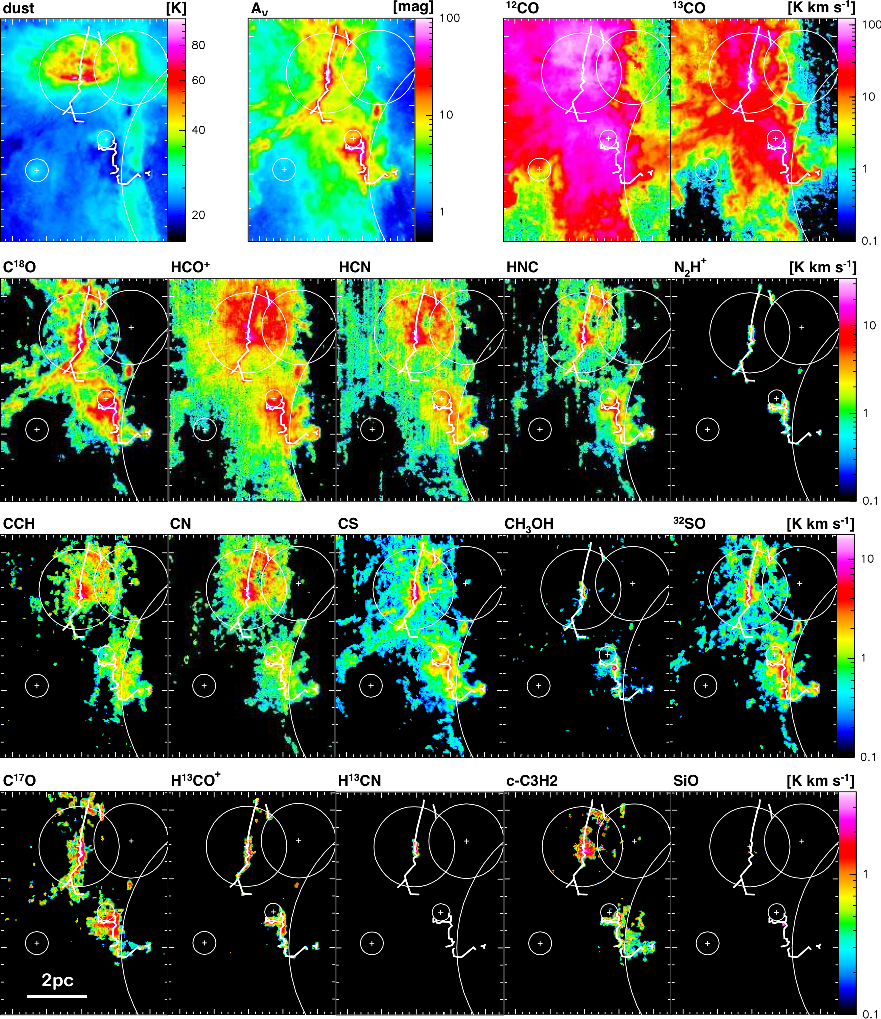
\includegraphics[width=\textwidth]{images/chapters/introduction/ism/Pety+16_overview.pdf}
    \caption[Distribution of molecules in Orion]{The distribution of molecules varies strongly within molecular clouds as shown here for Orion B \citep[adapted from figure 2]{2017A&A...599A..98P}. Less dense gas traced by CO is widespread around the central ridges seen in optical extinction (A$_\mathrm{v}$). The CO isotopologs $^{13}$CO, C$^{18}$O and C$^{17}$O are less and less abundant and trace increasingly dense regions within the cloud. The classical high density tracers HCN and HCO$^+$ are brightly detected over larger area of the cloud but other tracers better show the (projected) structures of the cloud internals. The shock tracer SiO is confined to one core and does not show in the rest of the cloud.}
    \label{introduction: figure: molecular cloud molecule distribution}
\end{figure}

The molecular content of a cloud is mainly H$_2$ by mass that survives dissociation by the shielding effect of outer layers of gas and dust. Towards the central regions, densities and path lengths to the outside increase, which is why more complex, less strongly bound and less abundant molecules are found there as shown in Figure~\ref{introduction: figure: molecular cloud molecule distribution} for a few tracers in the giant molecular cloud \ngc6334 \citep{2017A&A...599A..98P}. The temperature accordingly decreases towards the center because radiative cooling is possible by escaping photons of infrared or sub-mm lines while external heating sources are shielded by upper cloud layers. When internal heating mechanism start (e.g. star formation, Chapter~\ref{introduction: chapter: star formation}), the temperature structure becomes more complex.

The basic cloud properties size, linewidth and column density were empirically found to be related by \citet{Larson:1981jm} in three so-called Larson laws. These scaling relations can be explained theoretically with the gravitational and hydrodynamic properties and were re-examined frequently over the past 40 years \citep[e.g.][; see Krieger et al. (2020b, submitted) for a longer, yet incomplete list]{1987ApJ...319..730S,2007prpl.conf...81B,2010A&A...519L...7L,Bolatto:2008iv}.
The relations have been interpreted as evidence that molecular clouds are self-gravitating, bound entities of molecular gas, sometimes confined by external pressure \citep[e.g.][]{Heyer:2009ii,2011MNRAS.416..710F}. The modern understanding of molecular clouds expands on this definition by acknowledging the more complex structure with higher density gas nested inside lower density gas in a hierarchy of substructure \citep[e.g.][]{2007ARA&A..45..565M}. Still today the definition of a ``cloud'' is often unclear and context dependent.
In this thesis, a molecular cloud should be understood as a concept of a (sub-)structured amount of molecular gas with variable appearance and properties.


After more than 50 years of observational and theoretical molecular cloud research, the lifetimes and stability of clouds is still unclear and not yet fully understood. The virial parameter $\alpha = 2T/W = 5\sigma^2 R/GM$ parametrizes the gravitational stability of a cloud of size $R$, mass $M$ and line width $\sigma$ by quantifying the ratio between kinetic energy $T$ and gravitational energy $W$ \citep[e.g.][]{1992ApJ...395..140B}. According to the virial theorem, $\alpha \LESSSIM 1$ means the gravitational binding energy dominates and the cloud collapses on the free-fall time scale $\tau_{ff} = \sqrt{\frac{3\pi}{32 \mathrm{G} \rho }}$ determined by the density $\rho$ if no other relevant forces are present, whereas for $\alpha \GTRSIM 1$, internal kinetic energy dominates and the cloud would disperse if not confined by external pressure or other forces. A cloud's development and ability to form stars by (partial) collapse is therefore crucially dependent on the environment \citep[e.g.][]{2013ApJ...779...45M}.

Today, molecular clouds are thought to be dynamically evolving objects that on short timescales accrete mass, get dispersed or form stars. Most modern estimates (observational and theoretical) yield short cloud lifetimes of typically a few tens of Myr
(e.g. \citealt{1980ApJ...238..148B,Meidt:2015ig,2018MNRAS.476.3688J,Kruijssen:2019ej}; also see the review by \citealt{2015ARA&A..53..583H} for a discussion of arguments for short vs. long lifetimes).

If a cloud or part of a cloud becomes self-gravitating and collapses, this process is described by the Jeans instability \citep{1902RSPTA.199....1J}. At the edge of stability/instability, hydrostatic equilibrium must apply which can be translated to a comparison of time scales. If the free-fall time $\tau_{ff}$ is shorter than sound crossing time $\tau_{sound} = R/c_s$, a compressive perturbation cannot be counteracted quickly enough by pressure to restore equilibrium and the cloud collapses. For $\tau_{ff} = \tau_{sound}$, an instability length scale $\lambda_J = c_s/\sqrt{G\rho}$ can be derived describing the typical sizes of molecular clouds at given density $\rho$. Although real clouds are not spherical but often form elongated filaments (for example due to shear), the argument roughly holds. These time scales are of the order one to several Myr for typical GMCs and shorter for lower mass clouds.

The simple picture of cloud collapse drawn by the Jeans instability ignores crucial properties of clouds: non-thermal motions (turbulence) within the gas, rotation or magnetic fields can influence the stability of clouds. The net effect (stabilizing vs. de-stabilizing) and the (relative) strength of these properties is actively discussed in the literature.
For instance, turbulence adds additional kinetic energy to the cloud that helps to counteract gravitational pressure and can stabilize massive or dense clouds that would otherwise collapse \citep[e.g.][]{2018ApJ...854..100M}. Although not obvious at first glance, magnetic fields are relevant for molecular clouds because even low ionization fractions of the gas allow magnetic coupling and flux freezing. Thus, magnetic fields add a positive internal pressure to a cloud \citep[e.g.][]{Pillai:2015gr}. Today, the concensus is that both turbulence and magnetic fields are relevant for cloud stability but the quantitative importance depends on the individual cloud and the environment (e.g. \citealt{2012ARA&A..50...29C,2016ApJ...832..143F} and the review by \citealt{,2004RvMP...76..125M}).

Although molecular clouds are nowadays considered relatively quickly evolving phenomena on timescales of Myr \citep[e.g.][]{2007prpl.conf...63B,Kruijssen:2019ej}, they appear static in observations over a human lifetime. Beginning and end of the turbulent\footnote{pun intended} life of a molecular cloud are therfore difficult to infer from observations.
Local enhancements of the gas density, that allow molecular clouds to form, can occur due to many mechanisms within galaxies; to name a few: local converging flows \citep[e.g.][]{2005A&A...433....1A}, spiral-arm induced instability \citep[e.g.][]{2002ApJ...577..206E}, gravitational instability \citep[e.g.][]{2010A&A...518L.102A} or magneto-Jeans instability \citep[e.g.][]{2002ApJ...581.1080K}. 
A cloud's death by mass loss, dispersion and/or ionization can be caused by internal star formation or proceed without any sign of star formation within the cloud. For instance, turbulence driven by feedback (Section~\ref{introduction: section: star formation: feedback}) from a nearby star formation region may heat up the cloud kinematically and disperse the molecular gas which then gets dissociated by energetic radiation and cosmic rays \citep[e.g.][]{1999RvMP...71..173H}. If the cloud instead collapses and forms stars, it will not survive for long after the onset of star formation because stellar feedback (e.g. shocks, jets and radiation) will attack the cloud from the inside and blow away the remaining gas (outflows, Section~\ref{introduction: section: star formation: outflows}). 
Molecular clouds are therefore a transient feature of the ISM but nonetheless extremely important as there is no star formation without molecular clouds.


%%%%%%%%%%%%%%%%%%%%%%%%%%%%%%%%%%%%%%%%%%%%%%%%%%%%%%%%%%%%%%%%%%%%%%%%%%%%%%%%%%%%%%%%%%%%%%%%%%%%

\section{Observing the molecular ISM}
\label{introdution: section: ism: observations}

Molecular hydrogen is unfortunately very difficult to observe directly \citep[e.g.][]{1966SSRv....5..419V} due the lack of a permanent dipole moment. Furthermore, the low temperatures in molecular clouds prevent \htwo from reaching detectable populations in excited electronic states. Warm \htwo sufficiently populates low excitation vibrational and rotational states that can be detected in the infrared but requires sensitive, typically space-based, instruments (e.g. Spitzer).
Upcoming extremely sensitive and well-shielded instruments (ELT, JWST) will allow for frequent direct detection of warm molecular gas \citep[e.g.][]{2016AAS...22740902T}.

Cold and faint molecular gas still requires observations of molecular tracers that are easier to detect.
Carbon monoxide (CO) is the primary tracer of molecular gas \citep[e.g.][]{1991ARA&A..29..581Y} since it is usually the most abundant molecule after \htwo, offers easily observable spectral lines and correlates with molecular gas mass.
Due to the simple linear structure of the CO molecule, and therefore symmetries in two axes, it's excitation is limited to only one mode of rotation and vibration. 
The rotational transitions $J \rightarrow J-1$ in the vibrational ground state $\nu=0$ between rotational states $J$ and $J-1$ are located at frequencies of $f = J \times 115.27$\,GHz and thus fall into the mm and sub-mm spectrum.
For the vibrational stretching mode $\nu=1$, the rotational excitation ladder is at slightly lower frequencies ($f = J \times 114.22$\,GHz) which allows to observe both vibrational states simultaneously for low rotational excitation and with modern wideband instruments.
Rotational states of CO can be excited at temperature of tens to several hundred Kelvin and densities $\GTRSIM 100$\,\pcm3.

Due to the high abundance and bright spectral lines, CO emission easily becomes optically thick. This poses several problems since every detected photon does not correspond to a single molecule anymore but photons get absorbed and re-emitted within the cloud before reaching the observer. Therefore, the observed CO intensity does not directly correspond to the mass or the column density of the emitting cloud. Theoretical calculations and empirical measurements of a conversion factor X (or $\alpha$) allow to relate column density (mass) to the observed intensity (luminosity) but introduce substantial uncertainties \citep[e.g.][]{2013ARA&A..51..207B}.
Isotopologs such as $^{13}$CO or C$^{17}$O instead of the most common $^{12}$C$^{16}$O are far less abundant and thus are often optically thin. In these cases, the observed intensity is a direct measure of the number of emitting molecules and hence the cloud mass.

The tracer properties of CO are limited when it comes to dense ($\GTR 10^{3-4}$\,\pcm3) or diffuse molecular gas.
Studies have revealed that a substantial amount of \htwo, up to 95\% in extreme cases, is not traced by CO because CO requires better shielding against dissociating radiation to form than \htwo \citep[e.g.][]{2010ApJ...716.1191W}. Consequently, this gas is called CO-dark gas \citep[e.g.][]{1988ApJ...326L..69L}. In recent years, ionized carbon (C$^+$) is discussed as a better tracer of the total molecular gas mass \citep[e.g.][]{2016A&A...593A..42T}.

Higher density molecular gas in cloud cores is better traced by more complex molecules that require higher densities to collisionally excite their rotational states such as HCN or HCO$^+$. Other common molecular tracers are N$_2$H$^+$ (dense gas), NH$_3$ (temperature), H$_2$O (warm gas), OH (diffuse molecular gas) or SiO (shocks). The details of their molecular tracer properties are debated for most molecules.
As of February 2020, a total of 218 different molecular species have been detected in space according to the Cologne Database for Molecular Spectroscopy \citep[CDMS\footnote{List of detected molecules: \url{https://cdms.astro.uni-koeln.de/classic/molecules}}][]{2005JMoSt.742..215M}


The sizes of molecular clouds range from GMCs at $\GTR 100$\,pc down to cloud cores ($\sim 1$ pc) in which proto-stellar objects form on sizes measured in astronomical units ($4.8\times 10^{-6}$\,pc). To resolve those cloud scales in the molecular tracers with spectral lines in the sub-mm to radio regime, the targets need to be near-by. In Galactic targets, simple single dish telescopes may suffice but when aiming for the vast range of environments found across other galaxies, interferometers are essential to reach the desired resolution. This technique to create virtual telescopes with km-sized apertures allows to overcome the fundamental resolution limits of single-dish telescopes: a resolution $\Theta \sim \lambda / D$ requires enormous apertures ($D$) for long wavelengths ($\lambda$).
Instead, for interferometers, only large spacings $b$ between, in comparison, small antennas is required to achieve a resolution $\Theta \sim \lambda / b$.
The Atacama Millimeter/Submillimeter Array (ALMA, Figure~\ref{introduction: figure: ALMA}) is the primary interferometer in the millimeter to submillimeter range and provides the majority of the data presented in this thesis.
Interferometry is highly complex in operation but also data calibration and imaging later on. 
The focus of this thesis is on the astrophysical implications, so we omit the details of interferometry here. Instead, this was already laid out in detail in my Bachelor's and Master's theses (Krieger 2013, 2016; Heidelberg University).

\begin{figure}
    \centering
    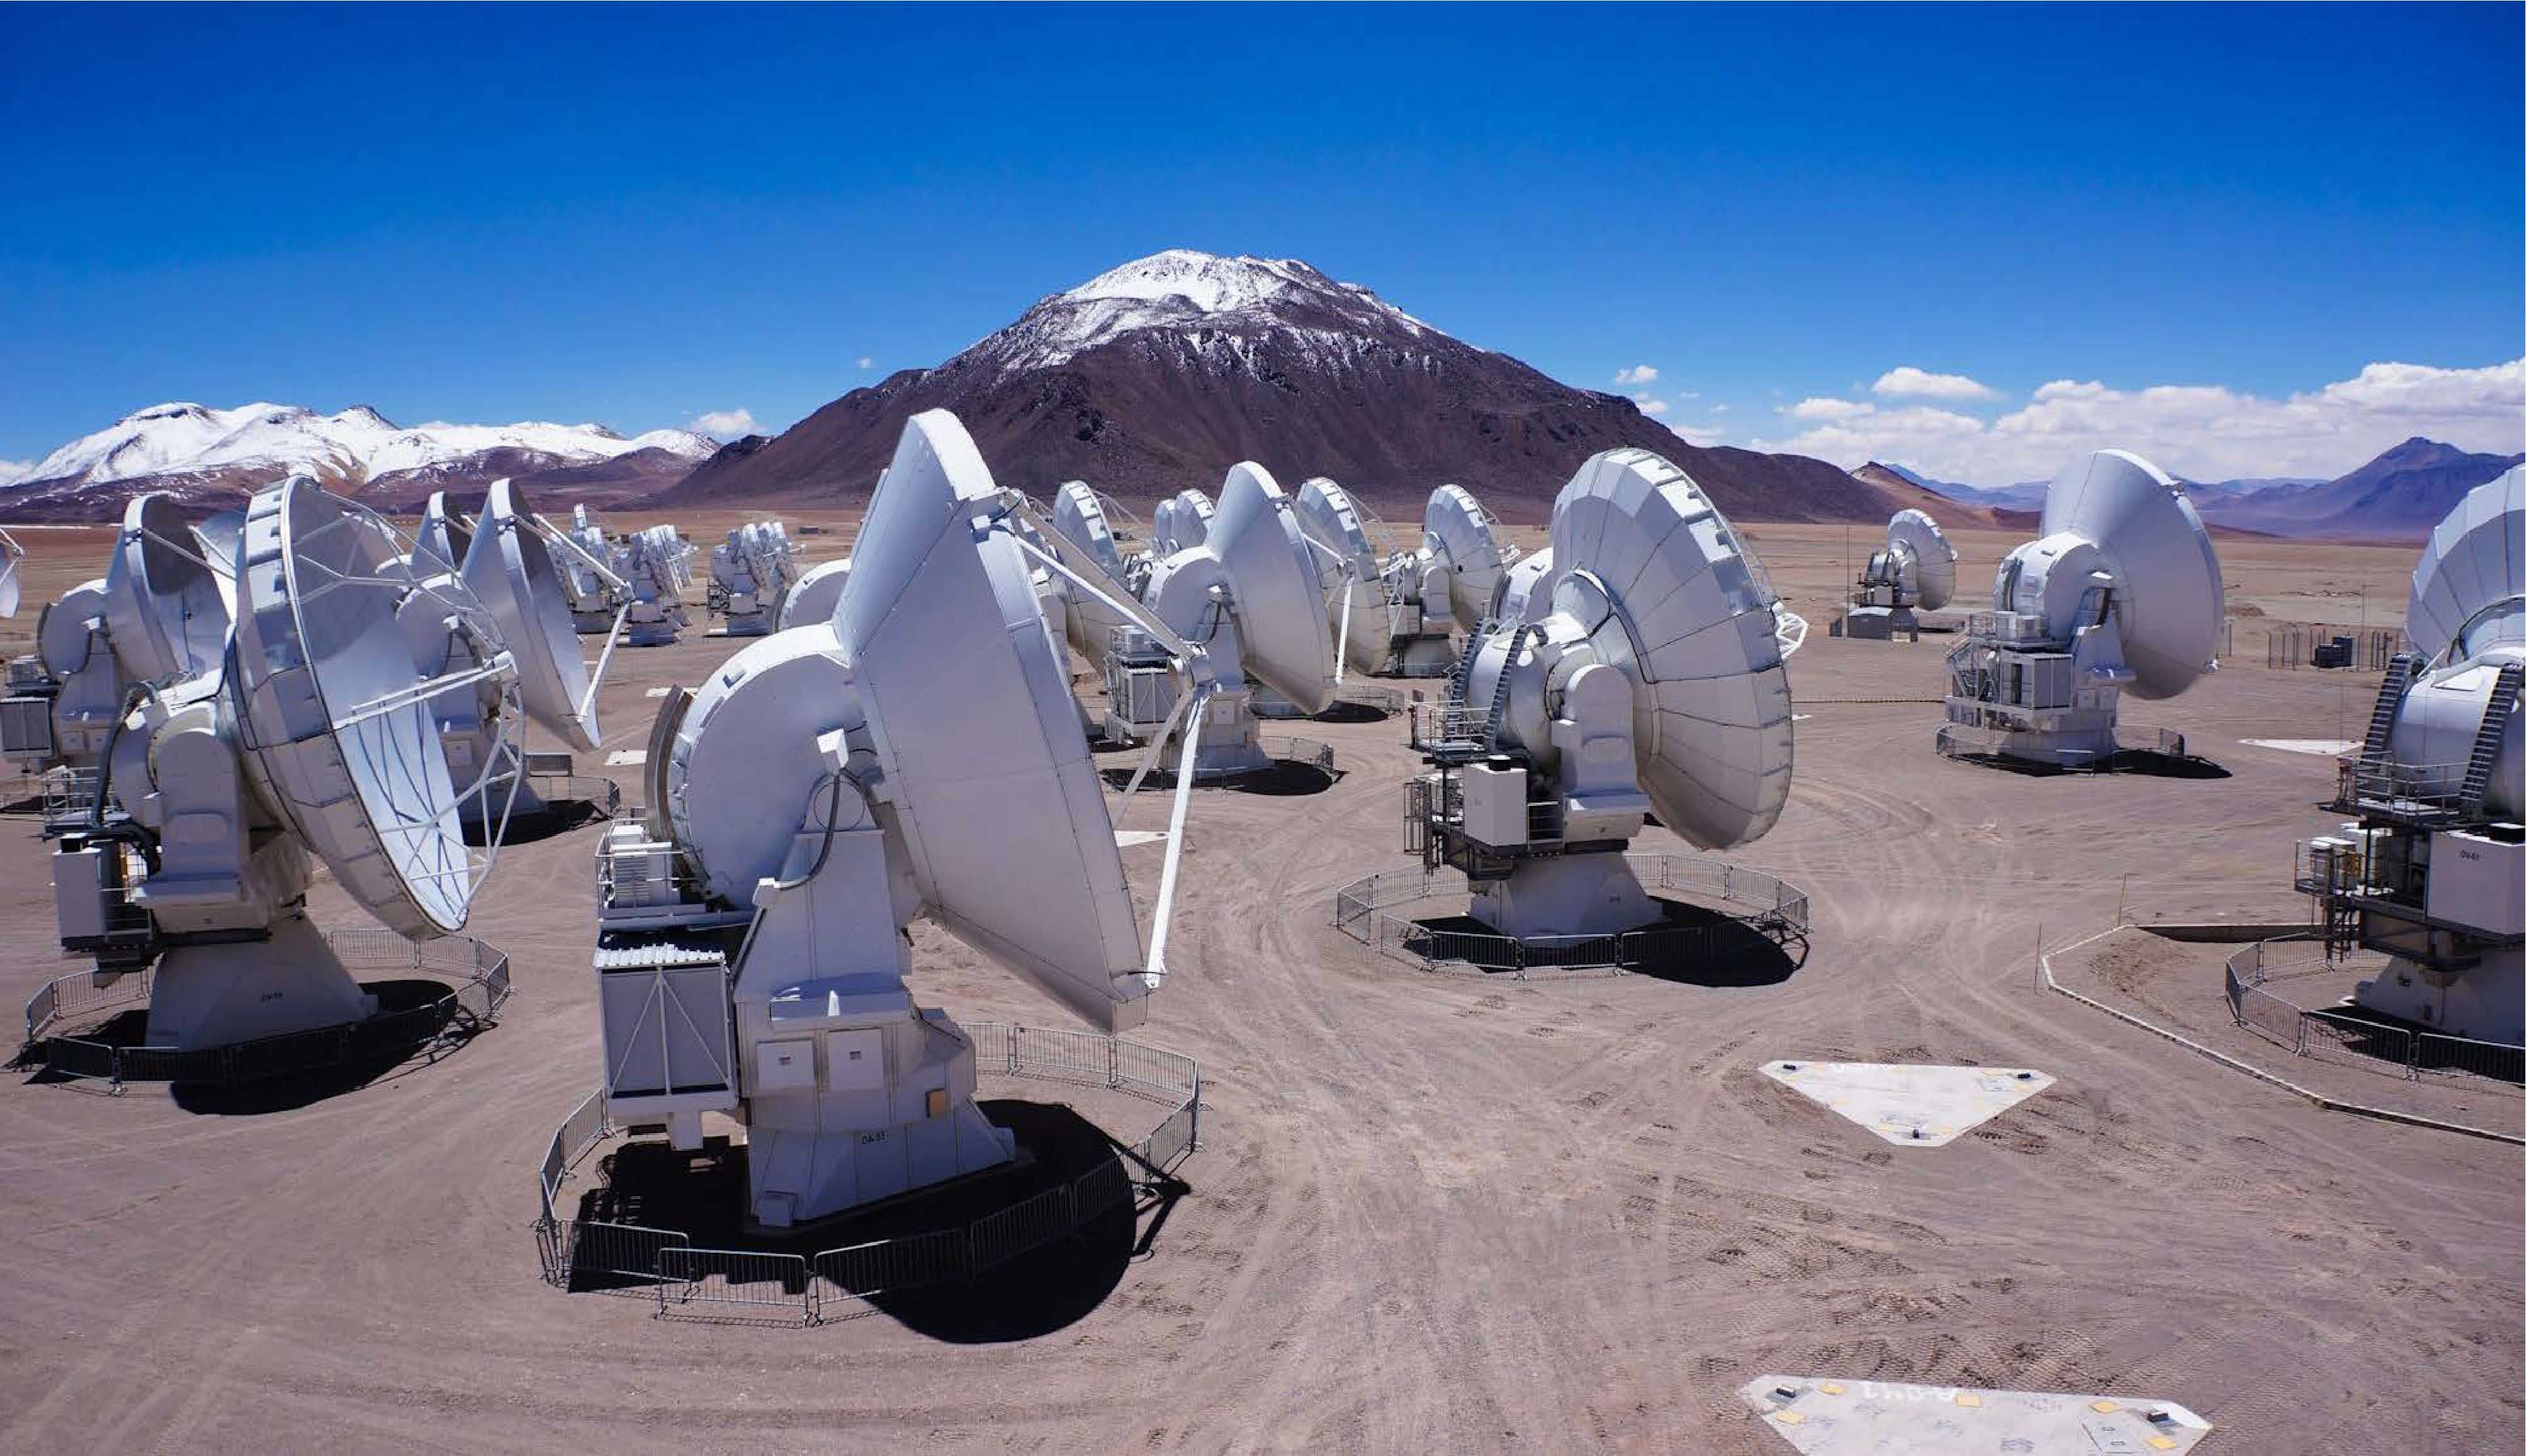
\includegraphics[width=\textwidth]{images/chapters/introduction/ism/ALMA_ACA_PCarrillo.pdf}
    \caption[Atacama Large Millimeter/Submillimeter Array]{View of the inner core of the Atacama Large Millimeter/Submillimeter Array (ALMA) on the Chajnantor plateau (Chile) with the Cerro El Chasc\`on (5703\,m) in the background. A total of 66 antennas ($12 \times 7$\,m diameter, $54 \times 12$\,m diameter) form the ALMA interferometer with baselines up to 16\,km. The combined collecting area allows for high sensitivity while the interferometer setup provides unprecedented resolution in the submillimeter wavelengths.
    Credit: NRAO, P. Carillo}
    \label{introduction: figure: ALMA}
\end{figure}

%%%%%%%%%%%%%%%%%%%%%%%%%%%%%%%%%%%%%%%%%%%%%%%%%%%%%%%%%%%%%%%%%%%%%%%%%%%%%%%%%%%%%%%%%%%%%%%%%%%%
